%%%%%%%%%%%%%%%%%%%%%%%%%%%%%%%%%%%%%%%%%%%%%%%%%%%%%%%%%%%%%%%%%%%%%%%%%%%%%%%%
%2345678901234567890123456789012345678901234567890123456789012345678901234567890
%        1         2         3         4         5         6         7         8

\documentclass[letterpaper, 10 pt, conference]{ieeeconf}  % Comment this line out if you need a4paper

% \documentclass[a4paper, 10pt, conference]{ieeeconf}      % Use this line for a4 paper

% \IEEEoverridecommandlockouts                              % This command is only needed if 
                                                          % you want to use the \thanks command

\overrideIEEEmargins                                      % Needed to meet printer requirements.

%In case you encounter the following error:
%Error 1010 The PDF file may be corrupt (unable to open PDF file) OR
%Error 1000 An error occurred while parsing a contents stream. Unable to analyze the PDF file.
%This is a known problem with pdfLaTeX conversion filter. The file cannot be opened with acrobat reader
%Please use one of the alternatives below to circumvent this error by uncommenting one or the other
%\pdfobjcompresslevel=0
%\pdfminorversion=4

% See the \addtolength command later in the file to balance the column lengths
% on the last page of the document

% The following packages can be found on http:\\www.ctan.org
%\usepackage{graphics} % for pdf, bitmapped graphics files
%\usepackage{epsfig} % for postscript graphics files
%\usepackage{mathptmx} % assumes new font selection scheme installed
%\usepackage{times} % assumes new font selection scheme installed
%\usepackage{amsmath} % assumes amsmath package installed
%\usepackage{amssymb}  % assumes amsmath package installed
\usepackage{amsfonts,amssymb} 
\usepackage{subfigure}
\usepackage{booktabs}
\usepackage{diagbox}
\usepackage{graphicx}
\usepackage{multirow}
\usepackage{amsmath}
\usepackage{overpic}
\usepackage{epstopdf}

\usepackage[linesnumbered,ruled,vlined]{algorithm2e}

\usepackage{caption}
\captionsetup{font={small}}

\usepackage{etoolbox}
\makeatletter
\patchcmd{\@makecaption}
{\scshape}
{}
{}
{}
\makeatother

\title{\LARGE \bf
3D Object Detection and Tracking on Streaming Data
}


\author{Xusen Guo$^{1}$ and Kai Huang$^{2}$% <-this % stops a space
% \thanks{*This work was not supported by any organization}% <-this % stops a space
% \thanks{$^{1}$Albert Author is with Faculty of Electrical Engineering, Mathematics and Computer Science, 
% University of Twente, 7500 AE Enschede, The Netherlands {\tt\small albert.author@papercept.net}}%
% \thanks{$^{2}$Bernard D. Researcheris with the Department of Electrical Engineering, 
% Wright State University, Dayton, OH 45435, USA {\tt\small b.d.researcher@ieee.org}}%
}

\def\eg{\emph{e.g.}}
\def\Eg{\emph{E.g.}}
\def\etal{\emph{et al. }}
\def\figurename{\emph{Figure}}
\def\tablename{\emph{Table}}

\begin{document}

\maketitle
\thispagestyle{empty}
\pagestyle{empty}


%%%%%%%%%%%%%%%%%%%%%%%%%%%%%%%%%%%%%%%%%%%%%%%%%%%%%%%%%%%%%%%%%%%%%%%%%%%%%%%%
\begin{abstract}

Recent approaches for 3D object detection have made tremendous progress due to the development of deep learning. However, previous researches are mostly single frame based, information between frames is scarcely explored. In this paper, we attempt to leverage the temporal information in streaming data and explore 3D object detection as well as tracking based on keyframes. Towards this goal, we set up a ConvNet architecture that can associate keyframes images and keyframes point clouds to generate accurate 3D detections and trajectories in an end-to-end form. Specifically, a tracking module is introduced to capture objects co-occurrences across time, and a motion based interpolation algorithm is proposed to generate streaming level results given keyframe detections. Our proposed architecture is proven to produce competitive results on the KITTI Object Tracking Benchmark, with 72.21\% in MOTA and 82.29\% in MOTP respectively.
\end{abstract}

%%%%%%%%%%%%%%%%%%%%%%%%%%%%%%%%%%%%%%%%%%%%%%%%%%%%%%%%%%%%%%%%%%%%%%%%%%%%%%%%
\section{INTRODUCTION}

3D Object detection has received increasing attention over the last few years due to the rapid development of autonomous driving. Compared to 2D image, 3D information can provide accurate localization of targets and characterize their shapes. Current approaches for 3D object detection are mostly carried out in three fronts: image based \cite{7780605, chen20183d}, point clouds based \cite{zhou2018voxelnet,yang2018pixor,simon2018complex}, and multi-view fusion based \cite{chen2017multi,ku2018joint}. Most of these approaches have achieved competitive results but are limited to single frame input.

During autonomous driving, data are always generated in a streaming fashion and thus it is more natural to perform object detection with streaming data. Compared to single frame, streaming data can provide consistent temporal correlations between consecutive frames for detected features, which can reduce detection noise over time. In addition, truncated and occluded targets can possibly be compensated by subsequent frames within streaming data. Therefore, exploring 3D object detection methods specifically for streaming data is essential and promising.

Performing 3D object detection in streaming data is however complex. First of all, acquiring consistent 3D information between frames is difficult. On the one hand, camera data provide rich appearance features but lack of depth information. On the other hand, though LiDAR can accurately detect the position of object of interest, it is very sparse and thus difficult to determine the appearance of object purely from its point cloud representation. Second, how to correlate the features between individual frames is not obvious. For example, generating 3D scene flow with temporal feature representation will need to determine the corresponding points between frames, which is not straightforward and challenging. Last but not least, the sheer numbers of frames that streaming data provided introduce unaffordable computational costs for frame level detection. 

This paper proposes a \textbf{D}ual-way \textbf{O}bject \textbf{D}etection and \textbf{T}racking network (\textbf{DODT}) to tackle the aforementioned problem. The intuition of our approach is that temporal features can be obtained through computing convolutional cross-correlation between adjacent frames, which has been demonstrated in \cite{feichtenhofer2017detect}. \textbf{DODT} consists of two detection branches, a \textit{shared RPN module} and a \textit{Tracking module}. Its structure is illustrated in \figurename \, \ref{fig:dodt}. Detection branches aggregate image features to compensate sparse point cloud data, thus can utilize the strengths if both. RPN module is feed with streaming data segment between two keyframes, and output 3D proposals shared by two detection branches. While \textit{Tracking module} utilizes correlation operation to encode temporal features and predict object displacements over frames, avoiding estimating 3D scene flow directly. Notably, different from \cite{feichtenhofer2017detect, dosovitskiy2015flownet}, our correlation is performed on proposal-level supported by sharing mechanism in RPN, which leads to a much lower computational cost. Note that the network is only performed on keyframes, thus we develop a motion based interpolation algorithm to propagate predictions to non-keyframes. Meanwhile, multi-object tracking can also be accomplished through \textit{tracking by detection} \cite{lenz2015followme}. Moreover, our interpolation algorithm shows a well solution for some common tracking problems such as drift, loss of targets in one frame, etc.

In summary, our contributions are threefold: \textit{(i)} We set up a dual-way network for 3D streaming-based object detection and multi-object tracking in autonomous driving scenarios. \textit{(ii)} We introduce a \textit{Tracking module} for temporal object cross-correlation representation, which is much efficient than previous approaches. \textit{(iii)} We develop a motion based interpolation algorithm for streaming level detection and multi-object tracking, which leads to considerable improvements on both tasks. 

%We perform our approach to KITTI Object Tracking Benchmark and obtain competitive results, with 72.21\% in MOTA and 82.29\% in MOTP respectively.

%The network has a RPN module to generate 3D proposals and two detection branches to perform 3D object detection on two adjacent keyframes respectively. To compensate for the sparsity of point cloud data, the network aggregates image features and thus can utilize the strengths of both. Considering the redundancy of features between frames, the 3D proposals are shared by two detection branches. In order to avoid estimating 3D scene flow directly when computing object cross-correlation features, a tracking module is aided to our network for temporal feature encoding. The tracking module uses correlation operation to extract temporal features and predict object displacements over keyframes, but different from traditional ways which performed on whole feature maps, it does correlation on object proposal-level with the help of sharing mechanism in proposals. 

%For a fast inference speed, we only performs object detection on keyframes and propagate predicted bounding boxes to neighboring frames for a streaming-based detection. By linking detections over time, multi-object tracking can be finished through \textit{tracking by detection} \cite{lenz2015followme}. Note that tracking using two frames often suffers from many problems, such as drift, loss of targets in one frame, etc. We develop a interpolation algorithm driven by motion model to address these problems. The ablation study shows the effectiveness of our interpolation algorithm.
%%%%%%%%%%%%%%%%%%%%%%%%%%%%%%%%%%%%%%%%%%%%%%%%%%%%%%%%%%%%%%%%%%%%%%%%%%%%%%%%
\begin{figure*}
	\vspace{-0.6cm}
	\rule{0pt}{1ex}
	%\setlength{\abovecaptionskip}{-0.1cm}
	\begin{center}
		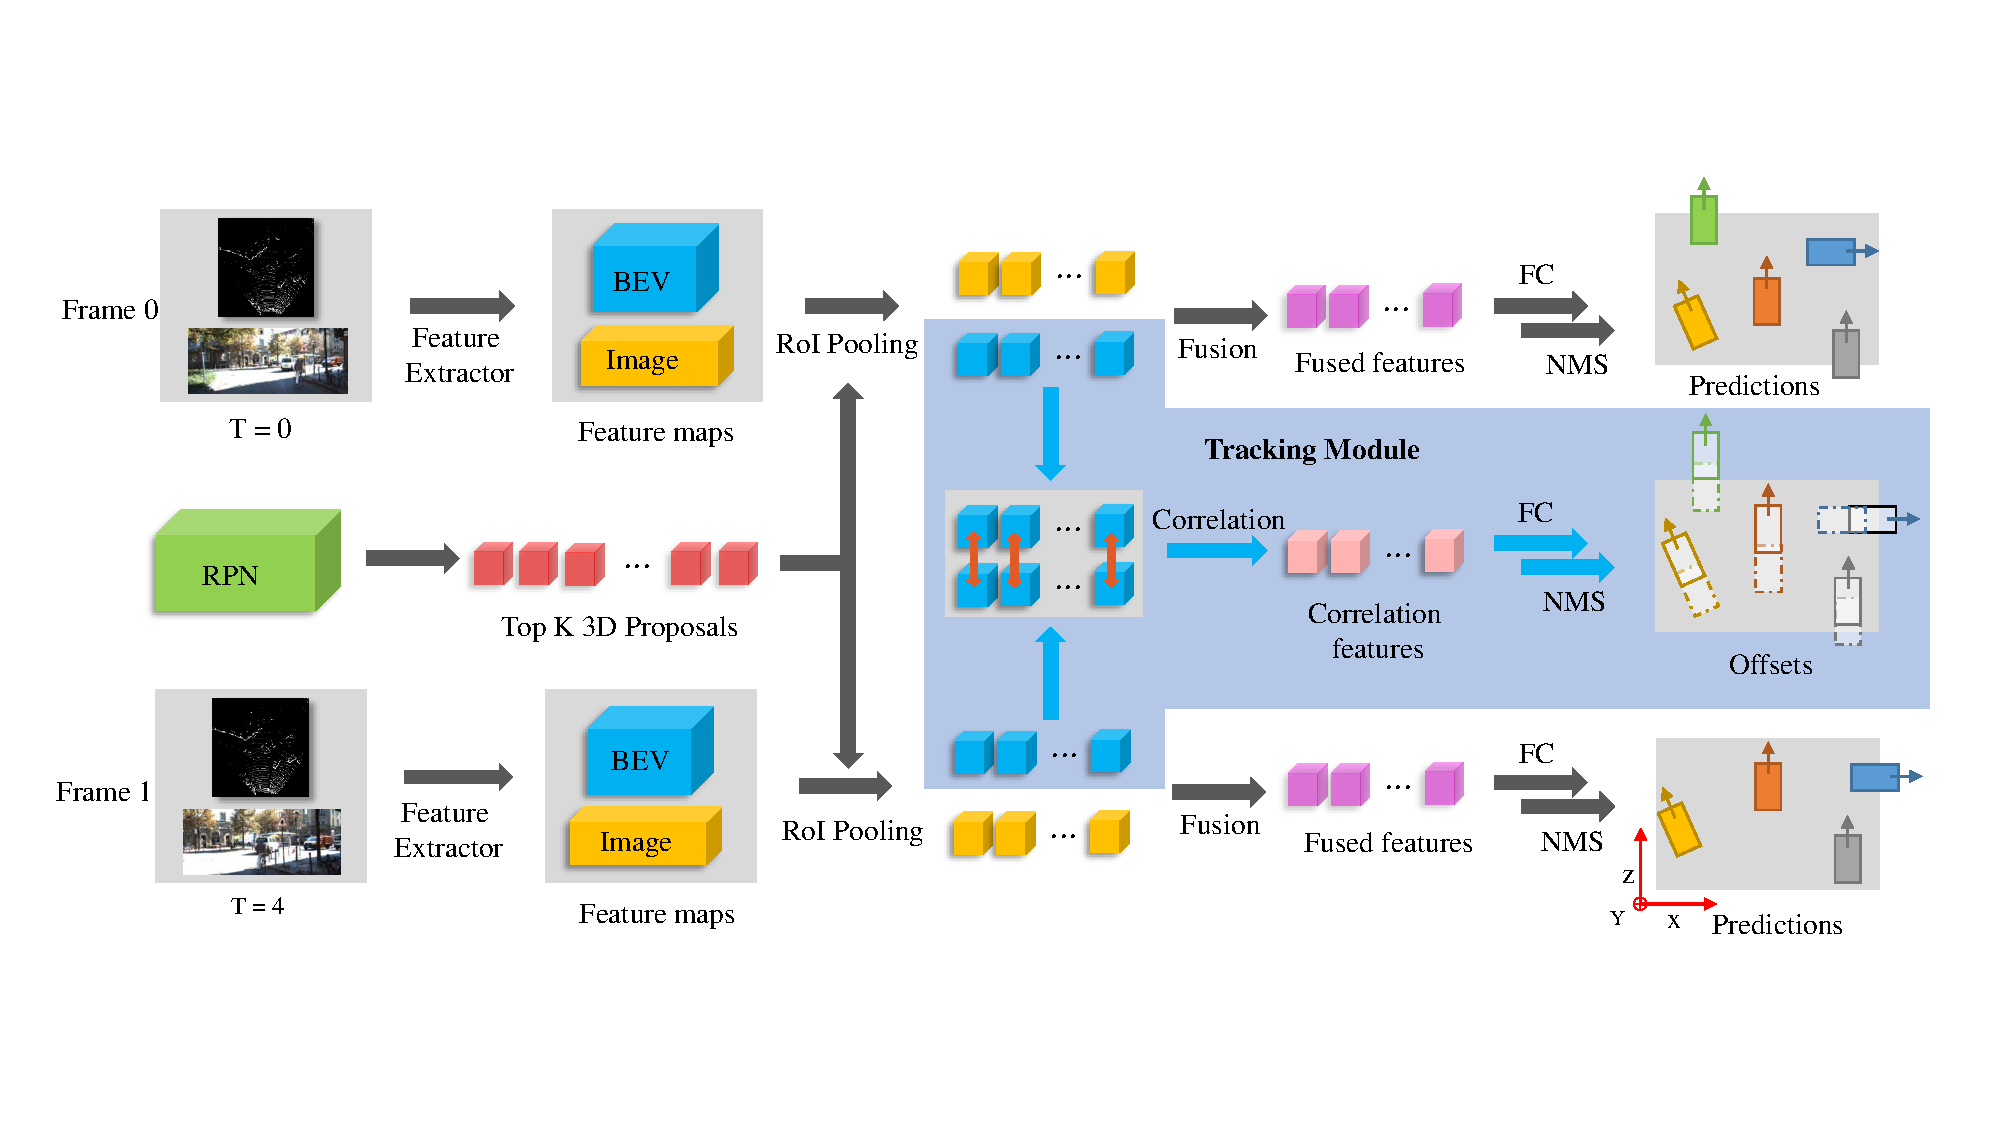
\includegraphics[trim={0.5cm, 3cm, 0.5cm, 3cm}, clip, width=\textwidth]{images/structure.pdf}
	\end{center}
	\caption{DODT architecture. Blue area is \textit{Tracking module}, it does not use image features since information in BEV is sufficient for tracking.}
	\label{fig:dodt}
	\vspace{-0.4cm}
\end{figure*}

\section{RELATED WORK}

\textbf{3D object detection.} Currently, most approaches in 3D object detection can be divided into three types: image based detectors, point cloud based detectors, and fusion based detectors. Image based approaches such as Mono3D \cite{7780605} and 3DOP \cite{chen20183d} use camera data only. Since image lacks depth information, hand-crafted geometric features are required in these approaches. Point cloud based methods are usually done in two fronts: voxelization based and projection based, according to how point clouds features are represented. Voxelization based methods such as 3D FCN \cite{li20173d}, Vote3Deep \cite{engelcke2017vote3deep}, VoxelNet \cite{zhou2018voxelnet}, utilize a voxel grid to encode features. These approaches suffer from the sparsity of point clouds and enormous computation costs in 3D convolution. While projection based methods such as PIXOR \cite{yang2018pixor}, Complex-YOLO \cite{simon2018complex}, Complexer-YOLO \cite{Simon_2019_CVPR_Workshops} attempt to project point clouds to a perspective view (e.g. bird eye view) and apply image-based feature extraction techniques. However, due to the sparsity of point cloud, features after projection are insufficient for accurate object detection, especially for small targets. Fusion based approaches such as F-PointNet \cite{qi2018frustum}, MV3D \cite{chen2017multi}, AVOD \cite{ku2018joint}, try to fuse point clouds with images to obtain accurate object detection. These methods distinguish from each other mainly on how data is fused. Our detection submodule is constructed based on AVOD, but proposal features are enhanced with temporal information additionally.

%first extracts the 3D bounding frustum of an object by extruding 2D bounding boxes from image detectors, then consecutively performs 3D object instance segmentation and amodal extent regression to estimate the amodal 3D bounding box. This method works well for indoor scenes and brightly lit outdoor scenes, but are expected to perform poorly in more extreme outdoor scenarios. MV3D \cite{chen2017multi} extends the image based RPN of Faster R-CNN\cite{ren2015faster} to 3D and proposes a 3D RPN, then applies feature fusion of images and point clouds to produces accurate 3D detections. However, due to the insufficient information in feature extraction caused by downsampling, it does not work well for small targets. AVOD \cite{ku2018joint} is similar to MV3D in 3D RPN and feature fusion, but with  full resolution feature maps produced by a pyramid architecture, which leads to a great improvement in localization accuracy for small targets. Our detection submodule is somehow similar to AVOD, but enhances proposal's feature with temporal information additionally.

\textbf{Video object detection.} Nearly all existing methods in video object detection incorporate temporal information on either feature level or final box level. FGFA \cite{zhu2017flow} leverages temporal coherence on feature level, it warps the nearby frames feature maps to a reference frame for feature enhancement according to flow emotion. On the other hand, T-CNN \cite{kang2018t, kang2016object} leverages precomputed optical flows to propagate predicted bounding boxes to neighboring frames, Seq-NMS \cite{han2016seq} improves NMS algorithm for video by constructing sequences along nearby high-confidence bounding boxes from consecutive frames. They are all utilize temporal information in final box level. There are also a few approaches attempt to learn temporal features between consecutive frames without optical flow. D\&T \cite{feichtenhofer2017detect} proposes a two branches detection network for object detection and tracking simultaneously in video. The network learns temporal information representation through computing convolutional cross-correlation between frames. Our DODT approach is mainly inspired by D\&T, however, we develop this idea to 3D space and restrain correlation operation in proposal-level, which reduce computational costs significantly. Moreover, tracking using two adjacent frames often suffers from drift, loss of targets in one frame, etc, our approach can handle these issues well by performing motion based interpolation algorithm.

%uses a detection and tracking based loss for simultaneous detection and tracking in video. In order to learn temporal information representation, the network is fed with multiple frames, and a correlation module is embedded for computing convolutional cross-correlation between frames. Our DODT approach is mainly inspired by D\&T, however, we develop this idea to 3D space. Moreover, we constrain correlation operation in proposal-level, which reduce computational costs significantly. 

%it first applies feature extraction network on individual frames to produce per-frame feature maps, and then enhances features at a reference frame by warping the nearby frames feature maps according to flow emotion. 
%On the other hand, final box level approaches usually utilize temporal information in bounding box post processing. T-CNN \cite{kang2018t, kang2016object} leverages precomputed optical flows to propagate predicted bounding boxes to neighboring frames, and then generates tubelets by applying tracking algorithms from high-confidence bounding boxes. Seq-NMS \cite{han2016seq} improves NMS algorithm for video by constructing sequences along nearby high-confidence bounding boxes from consecutive frames. While boxes of the sequence are then re-scored to the average confidence and other boxes close to this sequence are suppressed. 

%Other approaches such as D\&T \cite{feichtenhofer2017detect} attempt to learn temporal features between consecutive frames to avoid using optical flow. D\&T \cite{feichtenhofer2017detect} uses a detection and tracking based loss for simultaneous detection and tracking in video. In order to learn temporal information representation, the network is fed with multiple frames, and a correlation module is embedded for computing convolutional cross-correlation between frames. Our DODT approach is mainly inspired by D\&T, however, we develop this idea to 3D space. Moreover, we constrain correlation operation in proposal-level, which reduce computational costs significantly. 

\textbf{3D multi-object tracking.} Existing 3D multi-object tracking approaches are mostly implemented based on tracking by detection. For example, FaF \cite{luo2018fast} jointly reasons about 3D detection, tracking and motion forecasting taking a 4D tensor created from multiple consecutive temporal frames. It can aggregate the detection information for the past $n$ timestamps to produce accurate tracklets. DSM \cite{frossard2018end} first predicts 3D bounding boxes in continuous frames and then associates detections using a \textit{Matching net} and a \textit{Scoring net}, which is similar to our approach. However, their 3D detector is directly single frame based approach MV3D \cite{chen2017multi}, temporal features between frames are mostly ignored. Moreover, their bounding boxes association is done by solving a linear program and is an offline version, while our tracking algorithm is an near online approach.

%%%%%%%%%%%%%%%%%%%%%%%%%%%%%%%%%%%%%%%%%%%%%%%%%%%%%%%%%%%%%%%%%%%%%%%%%%%%%%%%

\section{METHODOLOGY}

In this section, we first give an overview of our DODT approach (Sec. A) that generates 3D object detection and tracking results given two adjacent keyframes as inputs. We then introduce the \textit{shared RPN module} (Sec. B) that predicts 3D proposals shared by two detection branches. Sec. C shows how \textit{Tracking module} encodes object co-occurrences and predicts the displacement of corresponding targets in two adjacent keyframes. Sec. D shows how we implement motion based interpolation algorithm to accomplish 3D streaming based object detection and multi-object tracking.

\subsection{DODT Model Structure} 

We aim at performing 3D object detection and tracking on streaming data. To this end, we design DODT architecture into a dual-way network. \figurename \, \ref{fig:dodt} illustrates the whole architecture. By doubling its inputs, we can feed two adjacent keyframes data simultaneously. The keyframes data consists of an image and point cloud BEV maps (following the procedure described in MV3D \cite{chen2017multi}). Keyframe data are first fed to feature extractors to get corresponding feature maps. The feature extractor is designed following the procedure described in AVOD \cite{ku2018joint}, which constructed in an encoder-decoder structure resulting in a full resolution feature map. To extract feature crops from image and BEV view feature maps, we also follow the idea proposed in AVOD. Given an 3D anchor generated by RPN, two view specific ROIs are obtained by projecting the anchor onto the BEV and image feature maps, the corresponding feature crops are extracted and then RoI pooling is performed from two views. After that, a \textit{early fusion} scheme is used to combine multi-view features in proposal-level. Finally, after fully connected layers and the non-maximum suppression (NMS) algorithm, the final detection outputs are produced. Meanwhile, fed with BEV feature crops of two branches, \textit{Tracking module} performs correlation operation to feature crop pairs to produce correlation features. The correlation features are then used to predict proposal-level offsets for streaming-level detection and tracking.

The whole network is designed in an end-to-end form. The multi-task loss consists of a cross-entropy loss $L_{cls}$ for classification, a smooth \textit{L1} loss $L_{reg}$ for coordinates regression, and a smooth \textit{L1} loss $L_{corr}$ for displacements regression between corresponding objects across two keyframes. $L_{reg}$ and $L_{corr}$ are normalized by the number of proposals while $L_{cls}$ is normalized by positive proposals.

\subsection{Shared RPN Module}

\begin{figure}
	\vspace{-0.6cm}
	\rule{0pt}{1ex}
	%\setlength{\abovecaptionskip}{-0.1cm}
	\begin{center}
		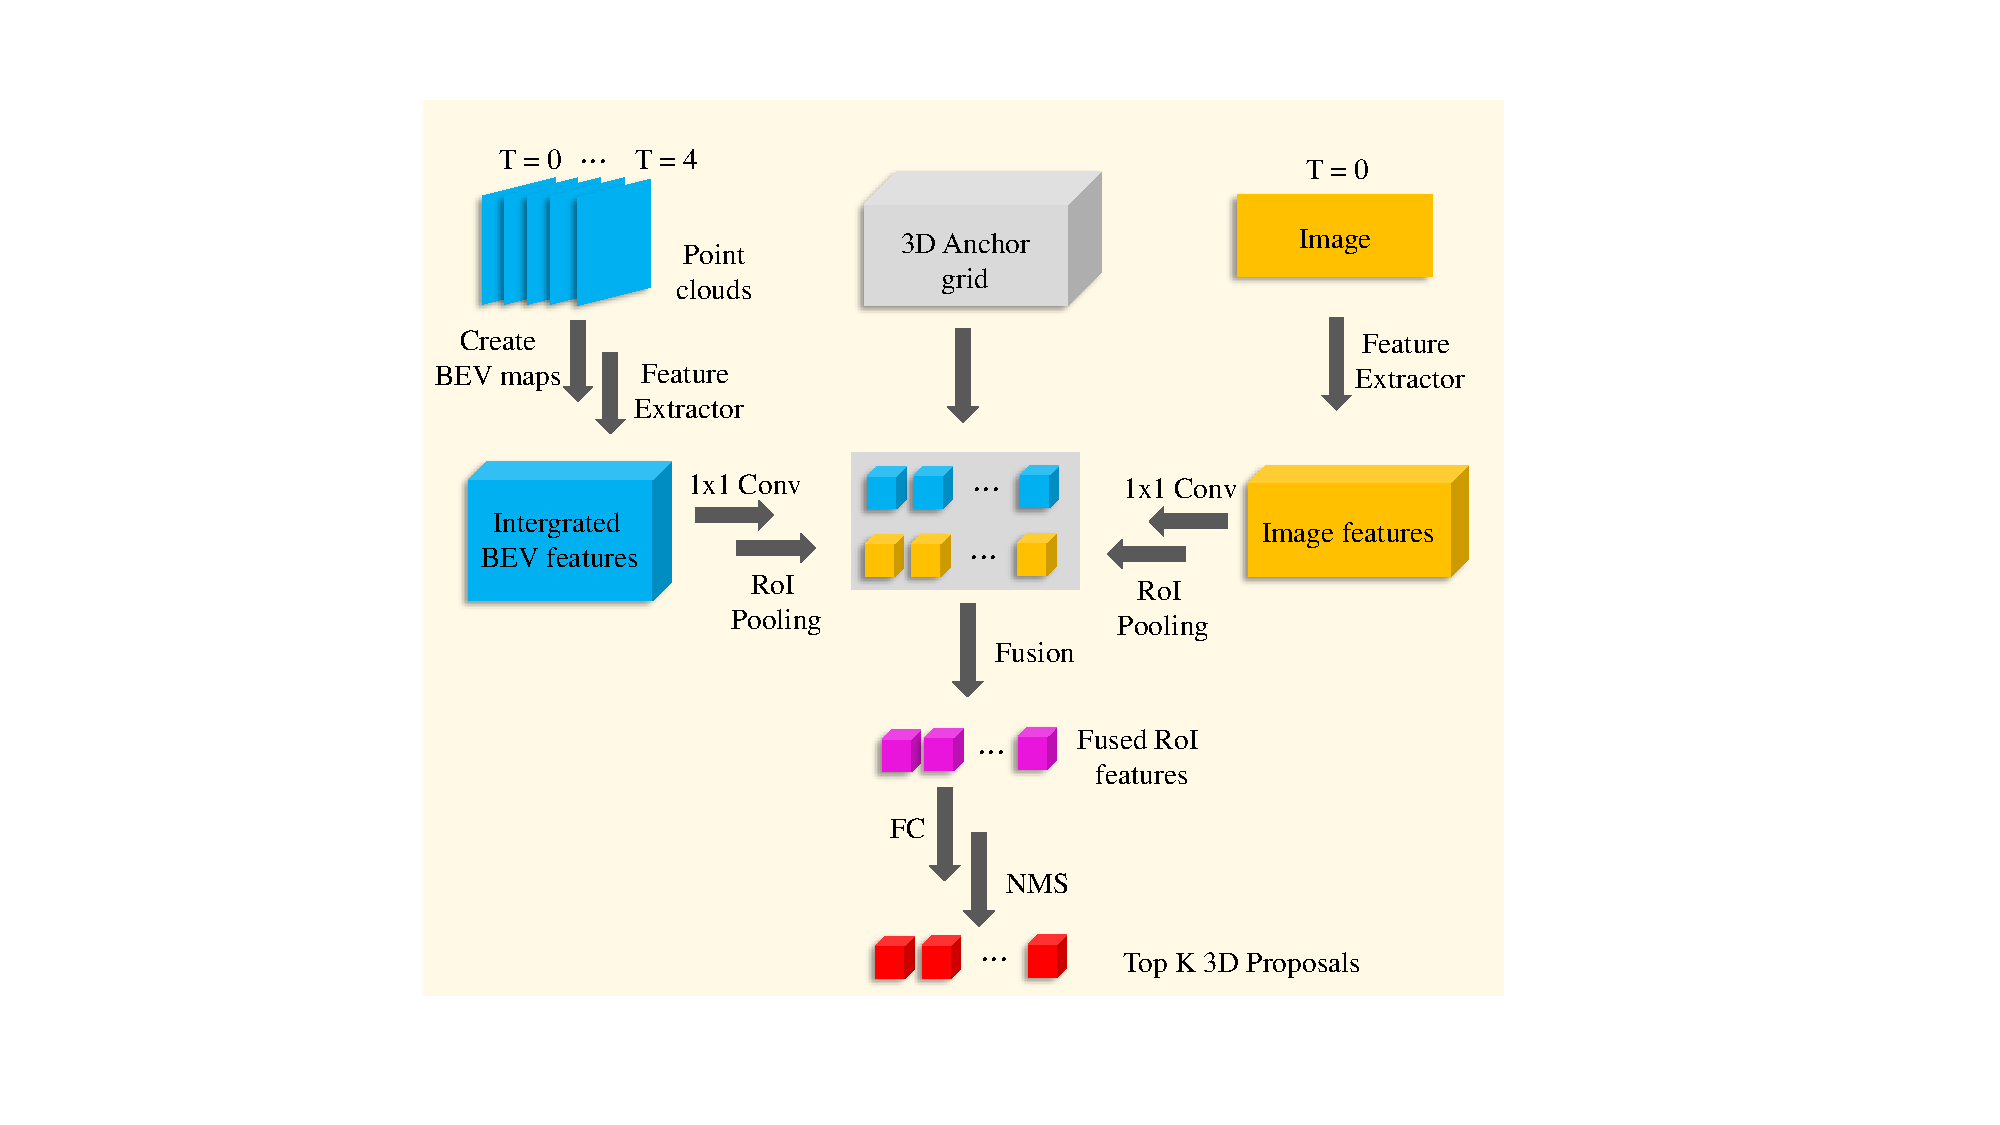
\includegraphics[trim={6.5cm, 2cm, 6.5cm, 2cm}, clip,width=0.5\textwidth]{images/rpn.pdf}
	\end{center}
	\caption{RPN structure.}
	\label{fig:rpn}
	\vspace{-0.5cm}
\end{figure}

We transform RPN network in AVOD \cite{ku2018joint} to our \textit{shared RPN network}, which can generate 3D proposals to both detection branches. The structure is shown in \figurename \, \ref{fig:rpn}. To ensure proposals generated by our RPN are suitable for both keyframes, we create integrated BEV feature maps based on frame segment between two keyfames. In this case is five consecutive frames. Note that point cloud shows object accurate 3D localization, we can simply transform five frames to a same coordinate system to fuse them. Since point cloud is extremely sparse and is encoded by projection, this process does not increase any computational cost but enhance the point cloud features. Due to object movement, the location of the same target in five frames are shift. For training convenient, we replace original labels with new axis-aligned labels that can cover all five original labels. \figurename \, \ref{fig:integrated_boxes} illustrates two kind of labels. Though this process enlarges proposal labels, it can ensure that new labels are suitable for proposals generation of both detection branches. To obtain accurate proposals, We fused image data to enhance object appearance features. Since one image contains enough features in a short temporal segment, our module only aggregates the features in first image of a segment. Subsequent processing and operations are similar with RPN module described in AVOD, we refer the reader to \cite{ku2018joint} for more information.

\begin{figure}
	\vspace{-0.6cm}
	\rule{0pt}{1ex}
	\begin{center}
		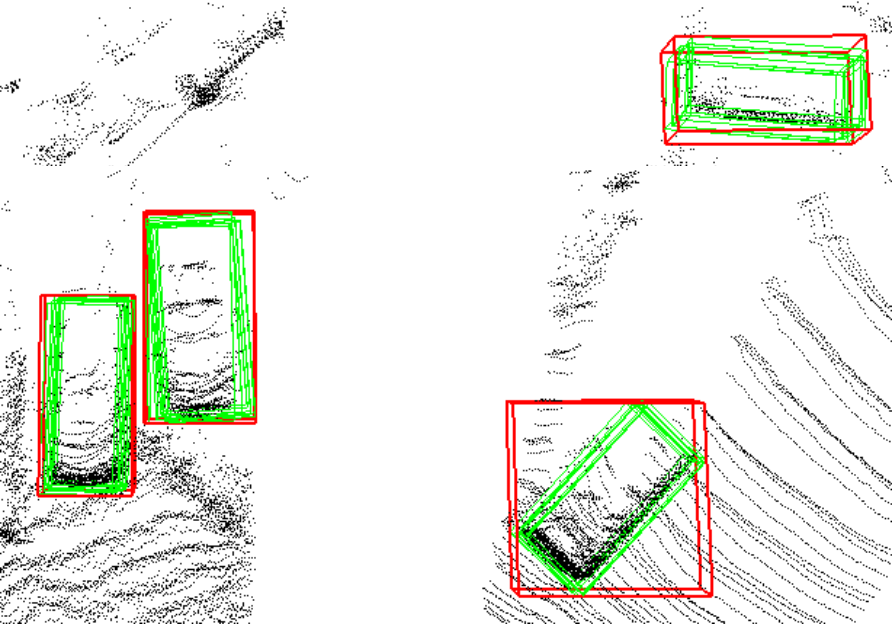
\includegraphics[width=0.4\textwidth]{images/integrated_boxes.png}
	\end{center}
	\caption{Five consecutive point clouds in the same coordinate system. Green boxes are default labels of five frames, while red boxes are the axis-aligned new labels for RPN training. The numbers are object id.}
	\label{fig:integrated_boxes}
	\vspace{-0.5cm}
\end{figure}

\subsection{Tracking Module}
The \textit{Tracking Module} is demonstrated in \figurename \, \ref{fig:dodt}. Given two sets of point cloud BEV features crops $F_t, F_{t+\tau}$, a set of cross frame feature pairs can be constructed as $\{(F_t^i, F_{t+\tau}^i)\mid i \in \{0,1,...,N\}\}$, where $F_t^i, F_{t+\tau}^i$ are features extracted by $i$-th proposal from frame $t$ and frame $t+\tau$ respectively, $\tau$ is temporal stride and $N$ is the number of 3D proposals. Note that the proposals generated by RPN are shared by two detection branches, thus the set can be obtained easily. After the correspondence of feature crops build, correlation operation is performed on feature pair $(F_t^i, F_{t+\tau}^i)$ to compute correlation features over frames. Once the correlation features are obtained, FC layers are used to predict the localization and shape offsets.

For a single target we have ground truth box $B^t = (B^t_x,B^t_z,B^t_l, B^t_w, B^t_{ry})$ in frame $t$, and similarly $B^{t+\tau}$ for frame $t+\tau$, denoting the horizontal and vertical center coordinates and its height, width as well as steering angle in BEV map. The tracking regression values for the target $\Delta^{t, t+\tau} = (\Delta^{t,t+\tau}_{x}, \Delta^{t,t+\tau}_{z}, \Delta^{t,t+\tau}_{l}, \Delta^{t,t+\tau}_{w}, \Delta^{t,t+\tau}_{ry})$ are then
\begin{equation}
\small
(\Delta_{x}^{t, t+\tau}, \Delta_{z}^{t, t+\tau}, \Delta_{ry}^{t, t+\tau}) = 
\begin{cases}
(\frac{B_{x}^{t+\tau} - B_{x}^{t}}{B^t_{w}}, \frac{B_{z}^{t+\tau} - B_{z}^{t} }{B^t_{l}}, \frac{B_{ry}^{t+\tau} - B_{ry}^{t}}{B^t_{ry}}) \\
\text{\qquad \qquad \qquad \qquad} B \in F_t \cap F_{t+\tau} \\
(0.0,0.0, 0.0) \text{\qquad \qquad }  else
\end{cases}
\end{equation}
\begin{equation}
\small
(\Delta_{l}^{t, t+\tau}, \Delta_{w}^{t, t+\tau}) = 
\begin{cases}
(0.0,0.0) & B \in F_t \cap F_{t+\tau} \\
(1.0, 1.0) & B \notin F_t \cap B \in F_{t+\tau} \\
(-1.0, -1.0) & B \in F_t \cap B \notin F_{t+\tau}
\end{cases}
\end{equation}
If the target exists in both keyframes, the shape offsets $(\Delta^{t,t+\tau}_{l}, \Delta^{t,t+\tau}_{l})$ are zero since 3D shape of vehicle dose not change over time. \textit{Tracking Module} only need to predict location offsets $(\Delta^{t,t+\tau}_{x}, \Delta^{t,t+\tau}_{z}, \Delta^{t,t+\tau}_{ry})$. If the target exists only in one keyframe, we set location offsets to zero but shape offsets to 1 for target appearance and -1 for disappearance. The encoding of object existence is the key technology to determine a birth or death of a trajectory, more details are available in Sec. D.


%Considering 3D shape of vehicle dose not change over time, and displacement information can be well represented by BEV feature maps, \textit{Tracking Module} only predicts X-axis, Z-axis offsets $(\Delta^{t,t+\tau}_{x}, \Delta^{t,t+\tau}_{z})$ of object center and steering angle  $\Delta^{t,t+\tau}_{ry}$. This is also why we use BEV feature crops only in \textit{Tracking Module}. In order to address object mismatch caused by tracklet birth or death, the module output a pair of offsets $(\Delta^{t, t+\tau},\Delta^{ t+\tau, t})$ corresponding to two keyframes. For an object exists only in one keyframe, its unique displacement can be used to determine whether a true start or end of a trajectory occurs, or just the instability of the model should be responsible for. More details are available in Sec. D.

\begin{figure}
	\vspace{-0.6cm}
	\rule{0pt}{1ex}
	\begin{center}
		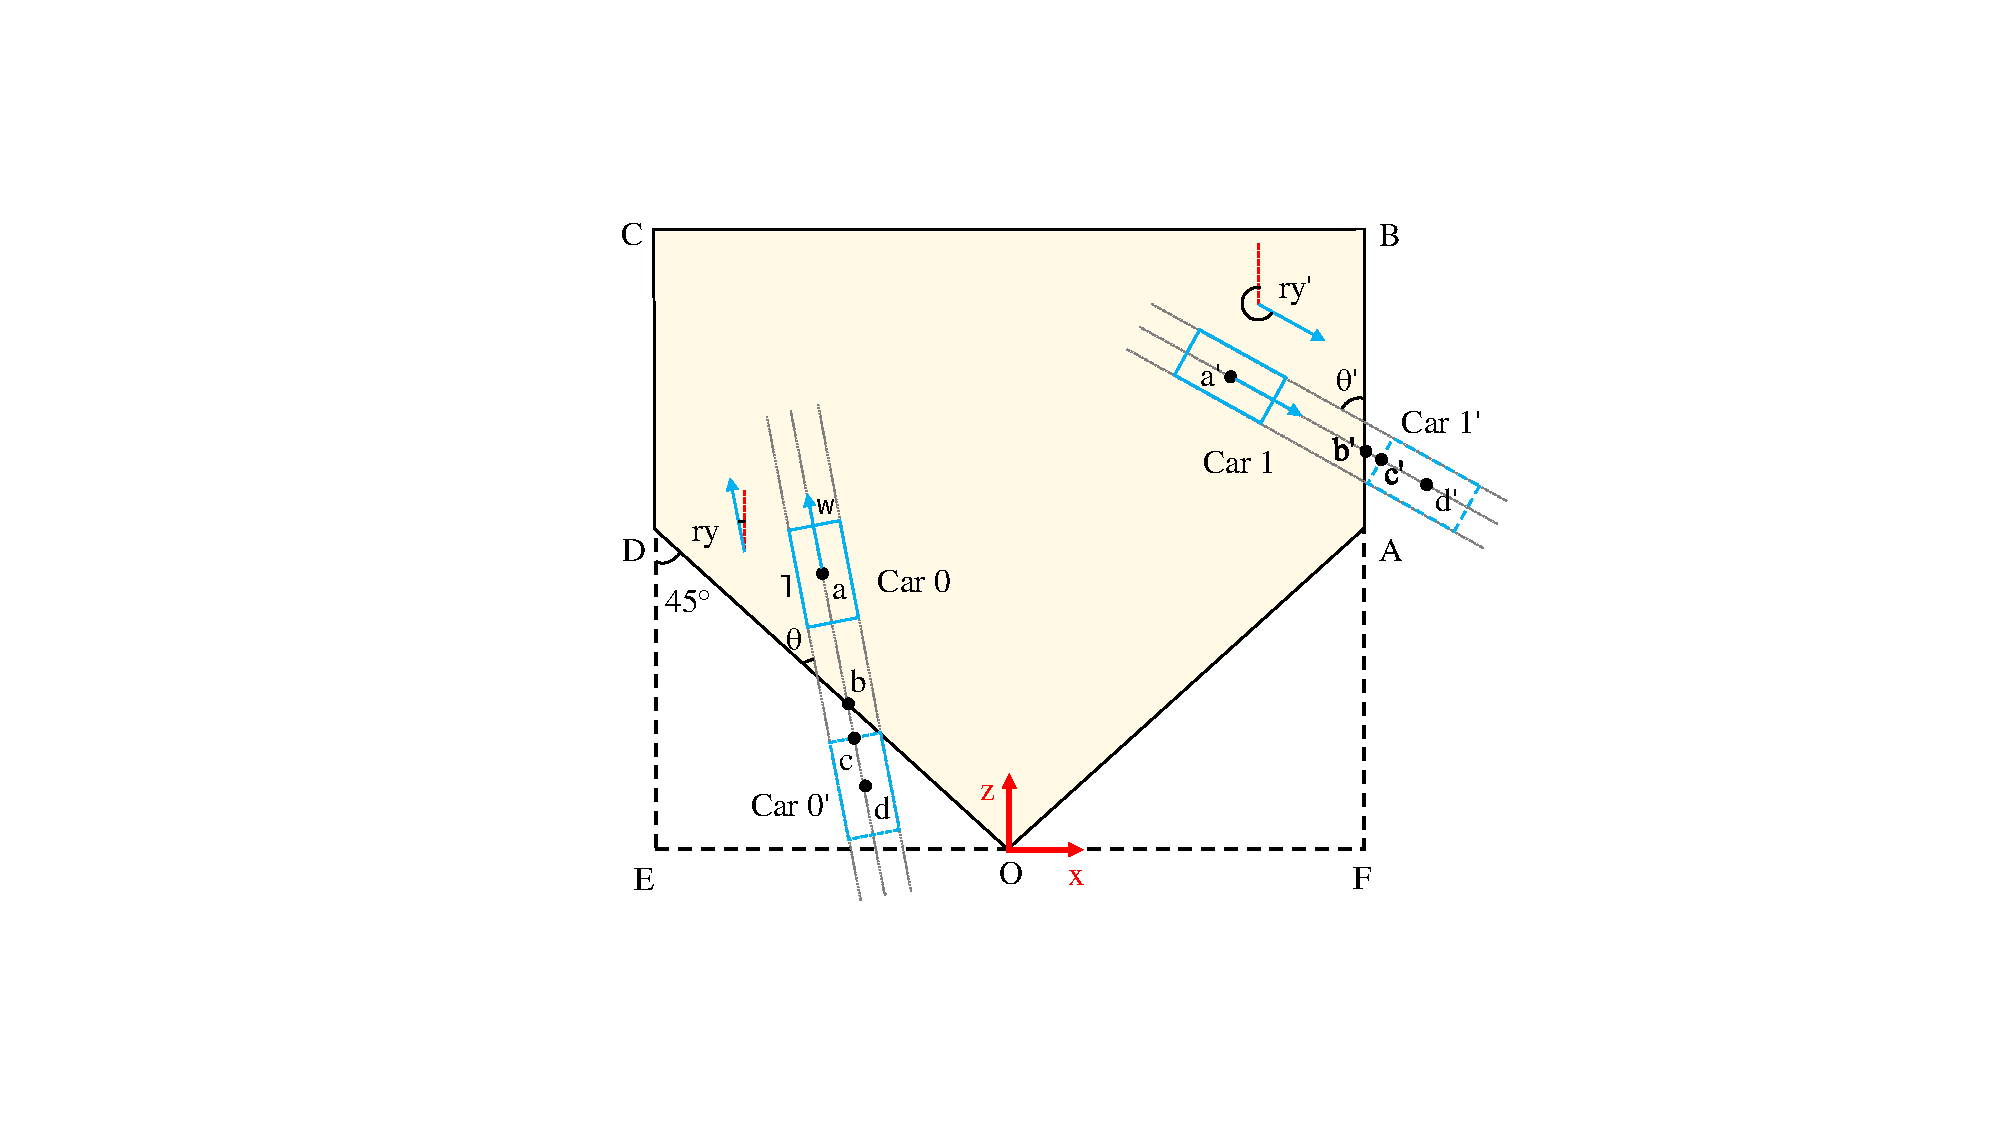
\includegraphics[trim={10cm, 4cm, 8cm, 3.5cm}, clip, width=0.5\textwidth]{images/motion.pdf}
	\end{center}
	\caption{Motion model of objects that in the start or end of a trajectory.}
	\label{fig:motion}
	\vspace{-0.6cm}
\end{figure}

\subsection{3D Streaming Object Detection and Tracking}
Since streaming data possesses a lot of redundant information and objects typically move smoothly in time, we can perform detection network on keyframes and compute detections of intermediate frames by applying \textit{Algorithm} \ref{alg:interpolation}. Fed with two detections lists and a offsets list, the algorithm first utilizes linear interpolation to calculate the detections in intermediate frames if an object exists on both keyframes. The co-occurrence is determined by a data association method named \textit{IsMatched}, which performs a IoU based algorithm to select the best matched detection in second keyframe given a rectified detection ($d_i^t + \delta_i^t$) in first keyframe. For a detection that exists only in one keyframe, if its absolute value of shape offsets $(\mid \delta^{t,t+\tau}_{i,l} \mid, \mid \delta^{t,t+\tau}_{i,w} \mid)$ are both less than $\delta_{max}$ (0.3 in our experiment), we assume a mis-detection in detection module, then we perform linear interpolation to compute detections. Otherwise we assume a trajectory birth or death appearance, then a motion model is leveraged to predict the detections.

The motion model is illustrated in \figurename \, \ref{fig:motion}. Rectangle BCEF is the range of selected point clouds with size of $[-40,40] \times [0, 70]$ meters along $X, Z$ axis respectively. While OABCD is the range contains points within the field of view of the camera. Taking $Car$ 0 as a example, it's a trajectory birth and is not detected in first keyframe, but is detected in second keyframe. We hold the hypothesis that $Car$ 0 is just outside OABCD and located in $d$ in first keyframe and its steering angle $ry$ is not change, thus the offset can be obtained by Equation (\ref{offsets}). Then the detections in intermediate frames can be calculated. Trajectory death case shows in $Car$ 1 can be handled in the similar way. 

Multi-object tracking can be accomplished with streaming level object detection simultaneously. Note that after performing interpolation algorithm on a keyframe pairs, data association between keyframe pairs is also obtained. We only need to associate keyframes detections to link tracklets in time and build long-term object tubes. This shows an near online tracking approach.

\vspace{-0.2cm}
\begin{equation}
\begin{split}
\mid ad \mid   &= \mid ab \mid + \mid bc \mid + \mid cd \mid  \\
&= \mid ab \mid + \frac{w}{2tan(\frac{\pi}{4} - ry)} + \frac{l}{2}
\end{split}
\end{equation}
\begin{equation}
\{\Delta_x, \Delta_z\} = \{\mid ad \mid sin(ry), \mid ad \mid cos(ry)\}
\label{offsets}
\end{equation}

%For multi-object tracking, we attempt to assign each detection in each frame to a unique trajectory utilizing an extended IOU tracker algorithm\cite{bochinski2018extending}. Unlike multi-object tracking in image which suffers from boxes overlap, detection in 3D has its unique position, any overlap of two detections in BEV means high probability of the same target. Thus a IOU based data association algorithm can also work well in our approach.

\begin{algorithm}[t]
	\small
	\caption{Motion based Interpolation Algorithm}
	\label{alg:interpolation}
	\textbf{Input: }$D^t= [d^t_0, d^t_1, ..., d^t_{N_t}], D^{t+\tau}= [d^{t+\tau}_0, d^{t+\tau}_1, ..., d^{t+\tau}_{N_{t+\tau}}],$
	$\Delta^t=[\delta^{t, t+\tau}_0, \delta^{t, t+\tau}_1, ..., \delta^{t, t+\tau}_{N}]$\\
	\textbf{Output: } $D = [D^t, D^{t+1}, ..., D^{t+\tau}]$\\
	\textbf{Initialize:} $D_{temp} = D^{t+\tau}, D, \delta_{max}$ \\
	\For{$d^t_i\in D^t$}{
		$d' = IsMatched(d^t_i+\delta^t_i, D_{temp})$\\
		\If{$d'$}{
			$d^{t+1}_i,..., d^{t+\tau-1}_i = Interpolate(d^t_i, d')$\\
			remove $d'$ from $D_{temp}$
		}
		\ElseIf{$|\delta^{t, t+\tau}_{i,l}| < \delta_{max} \text{ and } |\delta^{t, t+\tau}_{i,w}| < \delta_{max}$}{
			$d^{t+1}_i,..., d^{t+\tau-1}_i = Interpolate(d^t_i, \delta^t_i)$
		}
		\Else{predict $(d^{t+1}_i,..., d^{t+\tau-1}_i)$ by motion model}
	}
	\If{$D_{temp}$ is not empty}{
		\For{$d^{t+\tau}_j \in D_{temp}$}{
			\If{$|\delta^{t, t+\tau}_{j,l}| < \delta_{max} \text{ and } |\delta^{t, t+\tau}_{j,w}| < \delta_{max}$}{
				$d^{t+1}_j,..., d^{t+\tau-1}_j = Interpolate(d^{t+\tau}_j, \delta^{t+\tau}_j)$
			}
			\Else{
				predict $(d^{t+1}_j,..., d^{t+\tau-1}_j)$ by motion model
			}
		}
	}
\end{algorithm}
\setlength{\textfloatsep}{2pt}% change space between algorithm

\begin{table*}\centering
	\small
	\resizebox{\textwidth}{!}{
		\begin{tabular}{ccccccccc}
			                               &\multicolumn{1}{c|}{}   & \multicolumn{3}{c|}{IoU = 0.5}  		         & \multicolumn{3}{c|}{IoU = 0.7}          &  \\ \midrule
			\multicolumn{1}{c|}{Models} & \multicolumn{1}{c|}{Methods}    & Easy     & Moderate   & \multicolumn{1}{c|}{Hard}     & Easy  & Moderate & \multicolumn{1}{c|}{Hard}    & FPS \\\midrule
			\multicolumn{1}{c|}{AVOD\cite{ku2018joint}}&\multicolumn{1}{c|}{-}     & 90.40 / 90.91  & 71.71 / 72.72 & \multicolumn{1}{c|}{71.33 / 72.72}  & 75.24 / 90.90 & 55.11 / 72.69 & \multicolumn{1}{c|}{48.58 / 72.66}   & 12.5\\
			\multicolumn{1}{c|}{DODT ($\tau$ = 0)}     &\multicolumn{1}{c|}{-}     & 90.13 / 90.91  & 80.00 / 81.79 & \multicolumn{1}{c|}{71.61 / 81.79}  & 76.00 / 90.90 & 57.23 / 81.73 & \multicolumn{1}{c|}{56.13 / 72.69}   & 12.5\\
			\multicolumn{1}{c|}{DODT*($\tau$ = 0)}     &\multicolumn{1}{c|}{-}     & 98.04 / 99.94  & 88.77 / 90.89 & \multicolumn{1}{c|}{88.55 / 90.88}  & 87.66 / 90.91 & 68.98 / 90.85 & \multicolumn{1}{c|}{68.32 / 90.84}   & 12.5\\ \midrule
			\multicolumn{1}{c|}{DODT*($\tau$ = 1)}     &\multicolumn{1}{c|}{T}     & 98.70 / 99.96  & 89.28 / 91.88 & \multicolumn{1}{c|}{89.06 / 91.87}  & 88.16 / 90.91 & 75.14 / 90.82 & \multicolumn{1}{c|}{73.98 / 90.80}   & 10\\
			\multicolumn{1}{c|}{DODT*($\tau$ = 1)}     &\multicolumn{1}{c|}{M} & 00.00 / 00.00  & 00.00 / 00.00 & \multicolumn{1}{c|}{00.00 / 00.00}  & 00.00 / 00.00 & 00.00 / 00.00 & \multicolumn{1}{c|}{00.00 / 00.00}   & 10\\
			\multicolumn{1}{c|}{DODT*($\tau$ = 1)}     &\multicolumn{1}{c|}{T + M} & 00.00 / 00.00  & 00.00 / 00.00 & \multicolumn{1}{c|}{00.00 / 00.00}  & 00.00 / 00.00 & 00.00 / 00.00 & \multicolumn{1}{c|}{00.00 / 00.00}   & 10\\ 
			\multicolumn{1}{c|}{DODT*($\tau$ = 2)}     &\multicolumn{1}{c|}{T + M} & 00.00 / 00.00  & 00.00 / 00.00 & \multicolumn{1}{c|}{00.00 / 00.00}  & 00.00 / 00.00 & 00.00 / 00.00 & \multicolumn{1}{c|}{00.00 / 00.00}   & 00\\
			\multicolumn{1}{c|}{DODT*($\tau$ = 3)}     &\multicolumn{1}{c|}{T + M} & 00.00 / 00.00  & 00.00 / 00.00 & \multicolumn{1}{c|}{00.00 / 00.00}  & 00.00 / 00.00 & 00.00 / 00.00 & \multicolumn{1}{c|}{00.00 / 00.00}   & 00\\
			\multicolumn{1}{c|}{DODT*($\tau$ = 4)}     &\multicolumn{1}{c|}{T + M} & 00.00 / 00.00  & 00.00 / 00.00 & \multicolumn{1}{c|}{00.00 / 00.00}  & 00.00 / 00.00 & 00.00 / 00.00 & \multicolumn{1}{c|}{00.00 / 00.00}   & 00\\
			\multicolumn{1}{c|}{DODT*($\tau$ = 5)}     &\multicolumn{1}{c|}{T + M} & 00.00 / 00.00  & 00.00 / 00.00 & \multicolumn{1}{c|}{00.00 / 00.00}  & 00.00 / 00.00 & 00.00 / 00.00 & \multicolumn{1}{c|}{00.00 / 00.00}   & 00\\\midrule
		\end{tabular}}
	%\setlength{\abovecaptionskip}{2pt}
	\caption{We report $AP_{3D}/AP_{BEV}$ (in \%) of the \textbf{Car} category on our KITTI tracking evaluation datasets, 
		corresponding to average precision of the bird’s-eye view and 3D object detection. T is \textit{Treacking Module}, M is \textit{motion based interpolation algorithm}. 
		 $*$ means the network was first pretrained on KITTI object detection datasets, and then fine-tuned on our tracking training datasets. $\tau$ is temporal stride.} 
	\label{table:result_detection}
	\vspace{-0.4cm}
\end{table*}

%%%%%%%%%%%%%%%%%%%%%%%%%%%%%%%%%%%%%%%%%%%%%%%%%%%%%%%%%%%%%%%%%%%%%%%%%%%%%%%%
\section{EXPERIMENTS}
\subsection{Datasets and Training}

\textbf{Datasets and Preprocessing.} We use KITTI object tracking Benchmark \cite{geiger2013vision} for evaluation. It consists of 21 training sequences and 29 test sequences with vehicles annotated in 3D. We split 21 training sequences into two parts according to their sequence number, odd numbered sequences for training and the rest for evaluation. For multi-object tracking evaluation, we train our model in all 21 training sequences. Similar to the data preprocessing in AVOD \cite{ku2018joint}, we crop point clouds at $[-40, 40] \times [0, 70] \times [0, 2.5]$ meters along $X, Z, Y$ axis respectively to contain points within the field of view of the camera. To make the system invariant to the speed of the ego-car, we calculate the displacement of the observer between different frames and translate the coordinates accordingly. Location and velocity information of the ego-car are available in IMU data.

\textbf{Training and testing.} We train our network for \textit{Car} category temporarily, following most of the super-parameter settings in AVOD \cite{ku2018joint} during training and testing. The network is trained for 120K iterations using an ADAM \cite{kingma2014adam} optimizer with an initial learning rate of 0.0001 that is decayed exponentially every 30K iterations with a decay factor of 0.8. The weights of $L_{cls}, L_{reg}, L_{corr}$ are 1.0, 5.0, 1.0 respectively. During proposal generation, anchors with IoU less than 0.3 are considered background and greater than 0.5 are objects. To remove redundant proposals, 2D NMS is performed at an IoU threshold of 0.8 in BEV to keep the top 1024 proposals during training, while at inference time, the top 300 proposals are kept.

\subsection{Results}
\textbf{Shared RPN.} To evaluate the performance of our \textit{Shared RPN}, we implement a non-shared version of RPN. It predicts proposals for each keyframes independently based on each feature maps. A comparison of proposal prediction accuracy between \textit{Non-shared RPN} and \textit{Shared RPN} is shown in \figurename \, \ref{table:rpn_result}. Result showing \textit{Shared RPN} outperforms \textit{Non-shared RPN} by 0.66\% indicates that the shared mechanism in RPN promotes the accuracy of proposal prediction. 
\begin{table}[h]\centering
	\vspace{-0.2cm}
		\begin{tabular}{ccc}
			\toprule[1pt]
			Method        & Non-shared RPN & Shared RPN  \\ \midrule
			Accuracy(\%)  & 97.81      & \textbf{98.47}       \\
			\bottomrule[1pt]
	\end{tabular}
	\caption{Comparison of proposal prediction accuracy.}
	\label{table:rpn_result}
	\vspace{-0.2cm}
\end{table}

\textbf{3D object detection.} The main results on 3d object detection are summarized in \tablename \, \ref{table:result_detection}. Several important trends can be observed: \textbf{1)} compared to original AVOD \cite{ku2018joint} model trained on tracking training datasets, our DODT model (without \textit{Tracking Module} and interpolation algorithm) shows improvements in all settings with IoU threshold 0.7. These improvements indicate that the introduction of dual-way structure and \textit{Shared RPN} contribute to detection performance significantly. \textbf{2)} Fine-tuned model outperforms model trained from scratch by a large margin, over 10\% in almost all settings. Since KITTI tracking datasets are similar with KITTI object detection datasets, transfer learning can improve model performance greatly. 

\textbf{Streaming level detection.} We first evaluate the effectiveness of \textit{Tracking Module} and our interpolation algorithm with temporal stride $\tau = 1$. The results are shown in \tablename \, \ref{table:result_detection}. It's observed that the introduction of these two modules both contribute to model performance significantly, especially in \textit{Moderate} and \textit{Hard} setting with a overlap of 0.7. \textit{Tracking Module} brings 6.16\% and 5.66\% gain, while interpolation algorithm xx\% and xx\% respectively. These significant improvements indicate that 

Secondly, We investigate the effect of multi-frame input during testing. Specifically, we focus on the effect of different temporal strides $\tau$  on inference accuracy and speed. Towards this goal, we train five models with $\tau = \{1, 2, 3, 4, 5\}$, and then link the predicted detections over time and generate detections in intermediate frame by box interpolation. Results are shown in \tablename \, \ref{table:result_detection}. DODT* ($\tau = 3$) achieves the best result among five models, with xx\% $AP_{3D}$ in \textit{easy} setting, xx\% $AP_{3D}$ in \textit{moderate} setting, xx\% $AP_{3D}$ in \textit{hard} setting. Compared with the based fine-tuned model DODT* ($\tau = 0$), the $AP$ scores of DODT* ($\tau = 3$) can be boosted significantly (e.g. 3D \textit{moderate} setting by xx\%, 3D \textit{hard} setting by xx\%, BEV \textit{moderate} setting by xx\%, BEV \textit{hard} setting by xx\%). This gain demonstrates that the detection of truncated and occluded targets can benefit from a large temporal stride. However, there is also a non-ignorable decay on the \textit{easy} setting (by -xx\%), we think it is mainly caused by the failed link at both ends of the trajectories (see Sec. 3.4 for detail). Moreover,  \tablename \, \ref{table:result_detection} shows that a too large $\tau$ leads to a significant decay of accuracy. This is straightforward as a larger temporal stride introduces more failed trajectories link.

We calculate the inference time in streaming level. Results in  \tablename \, \ref{table:result_detection} shows that a larger temporal stride leads to less time cost per frame. Moreover, when $\tau$ is larger than 3, our Bi-AVOD network can run faster than origin AVOD in streaming level. We chose $\tau = 3$ for our following experiment, which is a good trade-off between speed and accuracy.

\begin{figure*}\centering
	\vspace{-0.6cm}
	\rule{0pt}{1ex}
	
	\begin{center}
		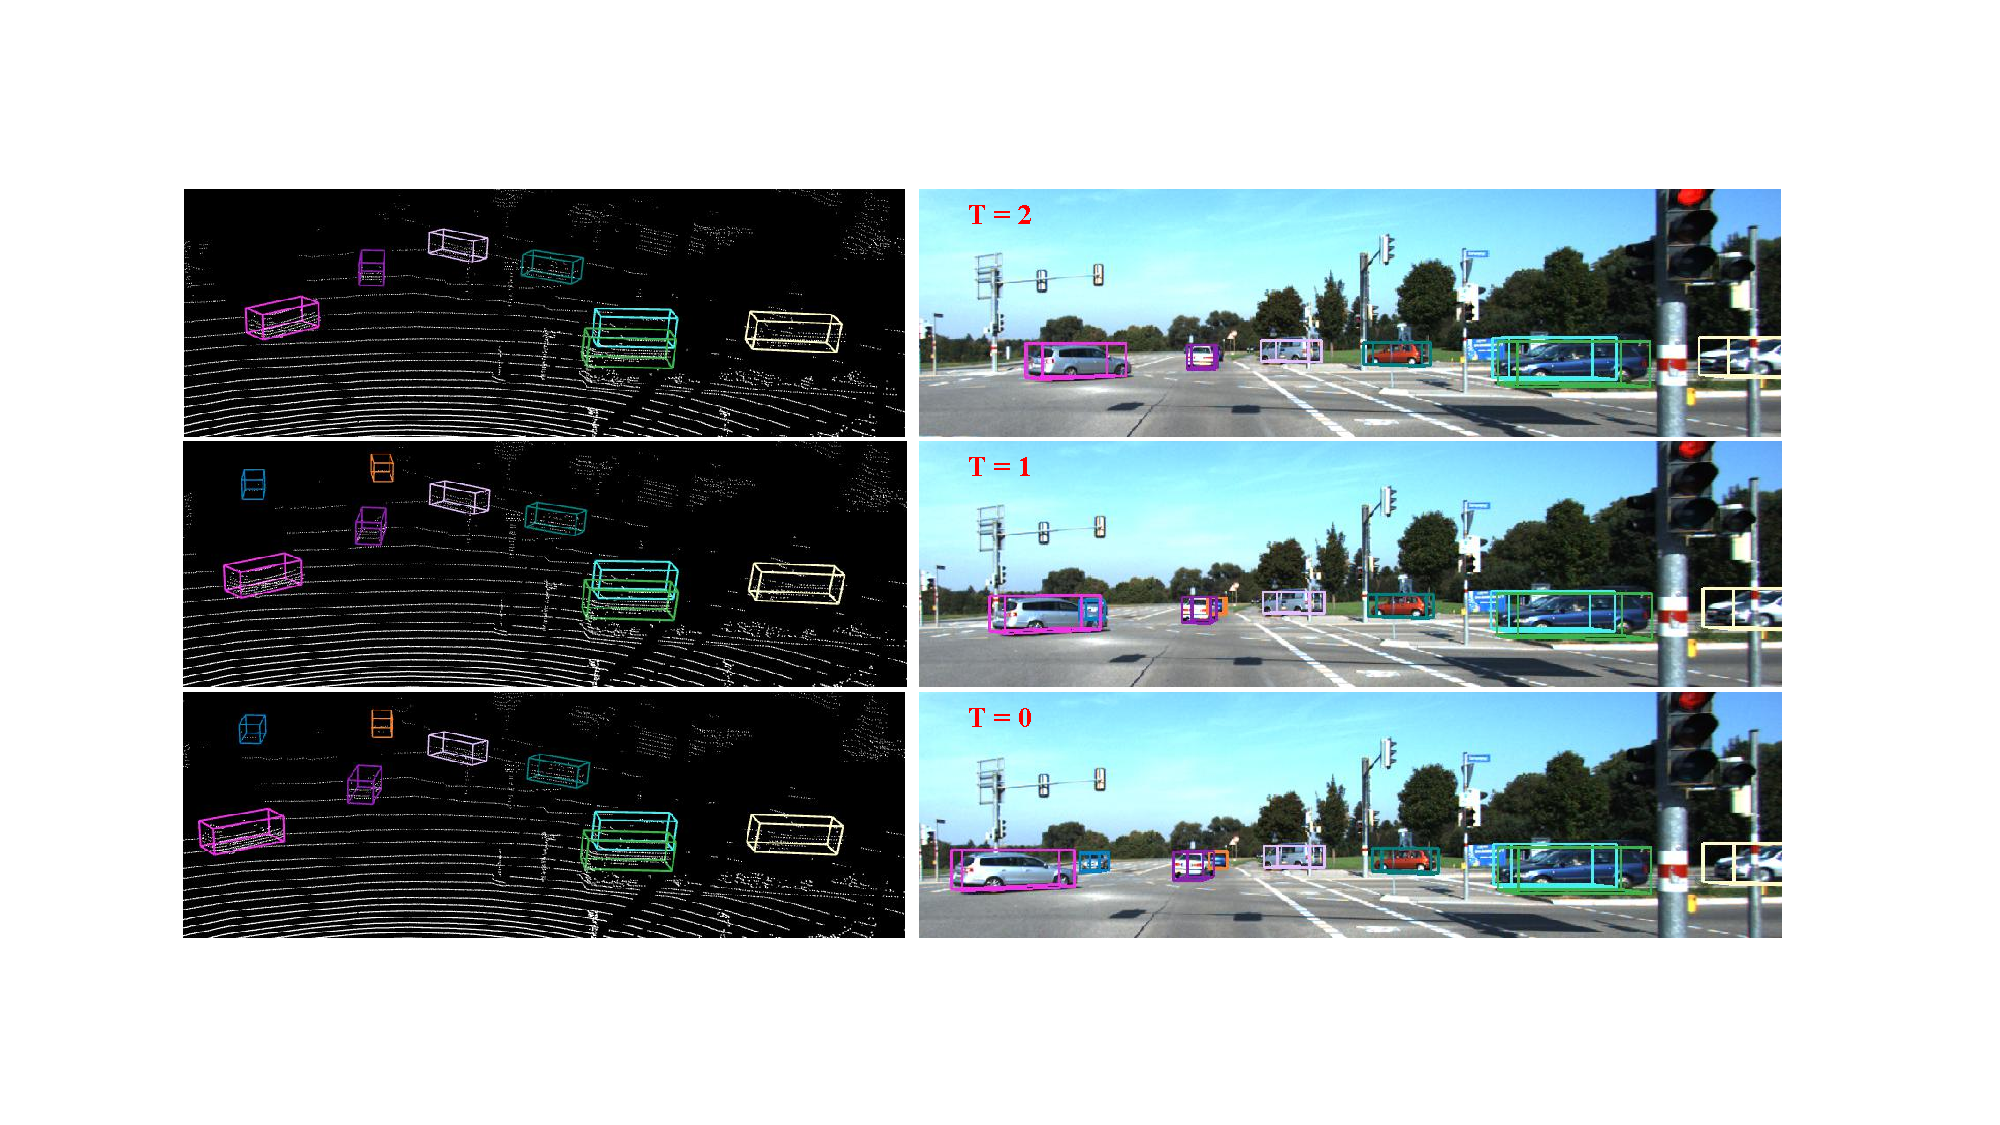
\includegraphics[trim={3cm, 3cm, 4cm, 3cm}, clip, width=\textwidth]{images/example.pdf}
	\end{center}
	\caption{Visualization of a set of trajectories produced by the tracker. Trajectories are color coded, such that having the same color means it's the same object.}
	%\setlength{\abovecaptionskip}{2pt}
	\label{fig:examples}
	\vspace{-0.4cm}
\end{figure*}

\begin{table}
	\resizebox{0.5\textwidth}{!}{
		\begin{tabular}{ccccccc}
			\toprule[1pt]
			Method        & MOTA(\%) & MOTP(\%) & MT(\%) & ML(\%) & IDS & FRAG \\ \midrule
			AVOD\cite{ku2018joint}          & 58.59    & 81.62    & 42.44  & 31.51  & \textbf{5}   & 166  \\
			DODT(ours) & \textbf{78.90}    & \textbf{84.22}    & \textbf{70.59}  & \textbf{5.04}  & 31  &  \textbf{123}  \\ 
			\bottomrule[1pt]
	\end{tabular}}
	\caption{Tracking performance comparison of origin AVOD and our Bi-AVOD on KITTI tracking evaluation datasets.}
	\label{label:result_tracking}
\end{table}

\begin{table}
	\resizebox{0.5\textwidth}{!}{
		\begin{tabular}{ccccccc}
			\toprule[1pt]
			Method        & MOTA(\%) & MOTP(\%) & MT(\%) & ML(\%) & IDS & FRAG \\ \midrule
			CEM\cite{Milan2014PAMI}           & 51.94    & 77.11    & 20.00  & 31.54  & 125 & 396  \\
			RMOT\cite{Yoon2015WACV}          & 52.42    & 75.18    & 21.69  & 31.85  & 50  & 376  \\
			TBD\cite{Geiger2014PAMI}           & 55.07    & 78.35    & 20.46  & 32.62  & 31  & 529  \\
			mbodSSP\cite{Lenz2015ICCV}        & 56.03    & 77.52    & 23.23  & 27.23  & \textbf{0}   & 699  \\
			SCEA\cite{Yoon2016CVPR}          & 57.03    & 78.84    & 26.92  & 26.62  & 17  & 461  \\
			SSP\cite{Lenz2015ICCV}            & 57.85    & 77.64    & 29.38  & 24.31  & 7   & 704  \\
			ODAMOT\cite{Gaidon2015BMVC}        & 59.23    & 75.45    & 27.08  & 15.54  & 389 & 1274 \\
			NOMT-HM\cite{Choi2015ICCV}       & 61.17    & 78.65    & 33.85  & 28.00  & 28  & \textbf{241}  \\
			LP-SSVM\cite{Wang2016IJCV}       & 61.77    & 76.93    & 35.54  & 21.69  & 16  & 422  \\
			RMOT*\cite{Yoon2015WACV}         & 65.83    & 75.42    & 40.15  & 9.69   & 209 & 727  \\
			NOMT\cite{Choi2015ICCV}          & 66.60    & 78.17    & 41.08  & 25.23  & 13  & 150  \\
			DCO-X*\cite{Milan2013CVPR}        & 68.11    & 78.85    & 37.54  & 14.15  & 318 & 959  \\
			mbodSSP*\cite{Lenz2015ICCV}       & 72.69    & 78.75    & 48.77  & 8.77   & 114 & 858  \\
			SSP*\cite{Lenz2015ICCV}           & 72.72    & 78.55    & 53.85  & \textbf{8.00}   & 185 & 932  \\
			NOMT-HM*\cite{Choi2015ICCV}      & 75.20    & 80.02    & 50.00  & 13.54  & 105 & 351  \\
			SCEA*\cite{Yoon2016CVPR}         & 75.58    & 79.39    & 53.08  & 11.54  & 104 & 448  \\
			MDP\cite{xiang2017subcategory}   & \textbf{76.59}    & 82.10    & 52.15  & 13.38  & 130 & 387   \\ \midrule 
			DODT(ours) & 72.21    & \textbf{82.29}    & \textbf{54.61}  & 15.38   & 113 & 523  \\ 
			\bottomrule[1pt]
	\end{tabular}}
	%\setlength{\abovecaptionskip}{1pt}
	\caption{Tracking performance comparison of publicly available methods in the KITTI Tracking Benchmark.}
	\label{label:result_kitti}
\end{table}

\textbf{Multi-object tracking.} We finally validate our approach on multi-object tracking. To investigate the effect of our correlation module, we compare our approach with original AVOD structure in our evaluation datasets. Performance comparison is shown in  \tablename \, \ref{label:result_tracking}. We see that Our Bi-AVOD approach outperforms origin AVOD by a large margin in nearly all tracking metrics (e.g. MOTA by 20.31\%, MOTP by 2.6\%, MT by 28.15\%, ML by 26.47\%, FRAG by 43). This indicates that our correlation module can improve the performance of multi-object tracking significantly. We also compare our approach to publicly available methods in KITTI Tracking Benchmark. In \tablename \, \ref{label:result_kitti} we see that our approach is competitive with the state of the art, outperforming other methods in some of the metrics (MOTP and MT). Note that KITTI only evaluates the metrics in 2D, which does not fully represent the performance of our 3D approach.
We also visualize some trajectories produced by our tracker. A example is shown in \figurename \, \ref{fig:examples}. It shows that our approach can generate nice trajectories for most targets, even though those truncated and occluded targets. More examples are available in the supplementary materials. 

%%%%%%%%%%%%%%%%%%%%%%%%%%%%%%%%%%%%%%%%%%%%%%%%%%%%%%%%%%%%%%%%%%%%%%%%%%%%%%%%

\section{CONCLUSIONS}

\label{sec:conclusions} We propose Bi-AVOD, a unified framework for simultaneous 3D object detection and tracking in streaming data. The network is a dual-way structure and can  process two frames at the same time. Embedded with a correlation module to encode the diversity of adjacent frames, our network can perform object detection and tracking in a very efficient way. Our approach achieves accuracy competitive with the state-of-the-art methods in KITTI Tracking Benchmark. In the future, we plan to improve our approach with a more flexible key frame selection algorithm and explore the mismatch problem of trajectory boundaries.

%%%%%%%%%%%%%%%%%%%%%%%%%%%%%%%%%%%%%%%%%%%%%%%%%%%%%%%%%%%%%%%%%%%%%%%%%%%%%%%%

\bibliographystyle{IEEEtran}
\bibliography{IEEEabrv,egbib}
\end{document}
